% ai-helper issue #46: the per-plane YZ-scaling simulation workflow for SBND
% (hand-off to the SBND calibration / YZ-map author).  FIRST-STAGE DRAFT: the
% workflow only; the 10-event BNB CV-like results are placeholders.
% Sources: ../yz-sim-kit/README.md (mtime 2026-11-24 23:34:09 -0600; sections 8
%   and 10 still had placeholders), the kit scripts/fcl/jsonnet,
%   ../46-sbnd-yz-depo-scaling.md (sections 1-3), WCT branch
%   sbnd-yz-depo-scaling (gen/src/DepoTransformYZ.cxx), and the kit-validation
%   outputs in /exp/sbnd/data/users/yuhw/YZ-non-uniformity/kit-validation.
% Style: same preamble as 46-yz-map-file-summary.tex.
% Build (twice): pdflatex 46-yz-sim-workflow.tex
\documentclass[aspectratio=169,10pt]{beamer}
\usetheme{default}
\setbeamertemplate{navigation symbols}{}
\setbeamertemplate{footline}{\hfill\scriptsize\color{gray}ai-helper \#46 \quad DRAFT \quad \insertframenumber/\inserttotalframenumber\hspace*{4mm}\vspace*{2mm}}
\setbeamertemplate{itemize items}{\textbullet}
\setbeamertemplate{itemize subitem}{--}
\setbeamerfont{frametitle}{size=\large,series=\bfseries}
\setbeamercolor{frametitle}{fg=black}
\setbeamercolor{structure}{fg=black!75}
\usepackage[T1]{fontenc}
\usepackage{lmodern}
\usepackage{booktabs}
\usepackage{array}
\usepackage{graphicx}
\usepackage{xcolor}
\usepackage{listings}
\usepackage{tikz}
\usetikzlibrary{arrows.meta,positioning,fit,calc,shapes.geometric}
\graphicspath{{deck-figs/}{../figs/}{workflow-figs/}}
\definecolor{open}{HTML}{B5470B}
\definecolor{yz}{HTML}{C0392B}
\definecolor{boxbg}{HTML}{F2F2F2}
\definecolor{todo}{HTML}{FFF4E0}
\newcommand{\open}[1]{\textcolor{open}{\textbf{#1}}}
\newcommand{\code}[1]{\texttt{#1}}
\setlength{\tabcolsep}{4pt}
% tighter lists
\makeatletter
\def\@listi{\leftmargin\leftmargini \topsep 2pt \parsep 0pt \itemsep 3pt}
\let\@listI\@listi
\def\@listii{\leftmargin\leftmarginii \topsep 1pt \parsep 0pt \itemsep 1pt}
\makeatother
\setlength{\leftmargini}{1.3em}
\setlength{\leftmarginii}{1.2em}

\lstset{basicstyle=\ttfamily\scriptsize, columns=fullflexible, keepspaces=true,
  backgroundcolor=\color{boxbg}, frame=none, xleftmargin=2pt, xrightmargin=2pt,
  aboveskip=2pt, belowskip=2pt, showstringspaces=false, breaklines=false,
  upquote=true}
\lstdefinestyle{diff}{moredelim=**[is][\color{yz}]{@+}{+@},
  moredelim=**[is][\color{gray}]{@-}{-@}}

% placeholder box
\newcommand{\placeholder}[1]{%
  \begin{center}\fcolorbox{open}{todo}{\parbox{0.92\textwidth}{\centering\vspace{2mm}%
  \open{To be filled after the 10-event run.}\\[1mm]\small #1\vspace{2mm}}}\end{center}}

\title{Per-plane YZ scaling in the SBND Wire-Cell simulation:\\workflow and how to run it}
\subtitle{DRAFT, first stage: the workflow. Results to follow.}
\author{ai-helper issue \#46}
\date{2026-11-25}

\begin{document}

% ---------------------------------------------------------------- 1
\begin{frame}
\titlepage
\vspace{-6mm}
\begin{center}\footnotesize\color{gray}
For the SBND calibration group (author of the YZ map).\\
Sources: the kit \code{yz-sim-kit/README.md} and its scripts; issue doc
\code{46-sbnd-yz-depo-scaling.md} sections 1--3;\\
WCT branch \code{sbnd-yz-depo-scaling}. Companion deck on the map file:
\code{46-yz-map-file-summary.pdf}.
\end{center}
\end{frame}

% ---------------------------------------------------------------- 2
\begin{frame}[fragile]{Goal and what changes physically}
\begin{columns}[T]
\begin{column}{0.5\textwidth}
\footnotesize
\textbf{Goal}: put the data's YZ non-uniformity of dQ/dx into the SBND MC, plane by plane.
\begin{itemize}
\item One factor per (plane, TPC, y, z) from the data map: $g = 1/C$, normalized to mean 1 per plane and TPC.
\item Applied to every energy deposit (depo), \textbf{per plane}, inside \code{DepoTransform}, before diffusion and the field/electronics response.
\item Why per plane: the planes differ as much as each plane varies (plane to plane 3--4.5\,\% rms; each plane 2.4--4.4\,\%; correlation 0.2--0.4). One factor per depo cannot do it (doc section 1).
\end{itemize}
\vspace{1mm}
\textbf{What does not change}
\begin{itemize}
\item SimChannels (true electrons): written before the scaling, the same in both modes.
\item Simulation cost: the same depo goes to all planes, only its charge changes. No extra cost expected (long-muon test: 4:55 vs 4:56 wall).
\end{itemize}
\end{column}
\begin{column}{0.48\textwidth}
\footnotesize
\textbf{The component}: \code{Gen::DepoTransformYZ}, a \code{DepoTransform} that overrides one hook. \code{DepoTransform} calls it for every depo and every plane before that plane's \code{BinnedDiffusion}.
\begin{lstlisting}
IDepo::pointer DepoTransformYZ::modify_depo(
        WirePlaneId wpid, IDepo::pointer depo)
{
  const auto& pos = depo->pos();
  const double scale = m_yzmap->value(
      m_key, wpid.index(), pos.y(), pos.z());
  if (scale == 1.0) return depo;
  return std::make_shared<Aux::SimpleDepo>(
      depo->time(), pos, depo->charge() * scale,
      depo, depo->extent_long(),
      depo->extent_tran(), depo->id(),
      depo->pdg(), depo->energy());
}
\end{lstlisting}
\vspace{1mm}
\begin{itemize}
\item \code{configure()} fails if the map has no non-zero value for a plane of the anode: a wrong key cannot silently zero the charge.
\item File: \code{gen/src/DepoTransformYZ.cxx} (code condensed here).
\end{itemize}
\end{column}
\end{columns}
\end{frame}

% ---------------------------------------------------------------- 3
\begin{frame}{Where it sits in the SBND chain}
\centering
\resizebox{\textwidth}{!}{%
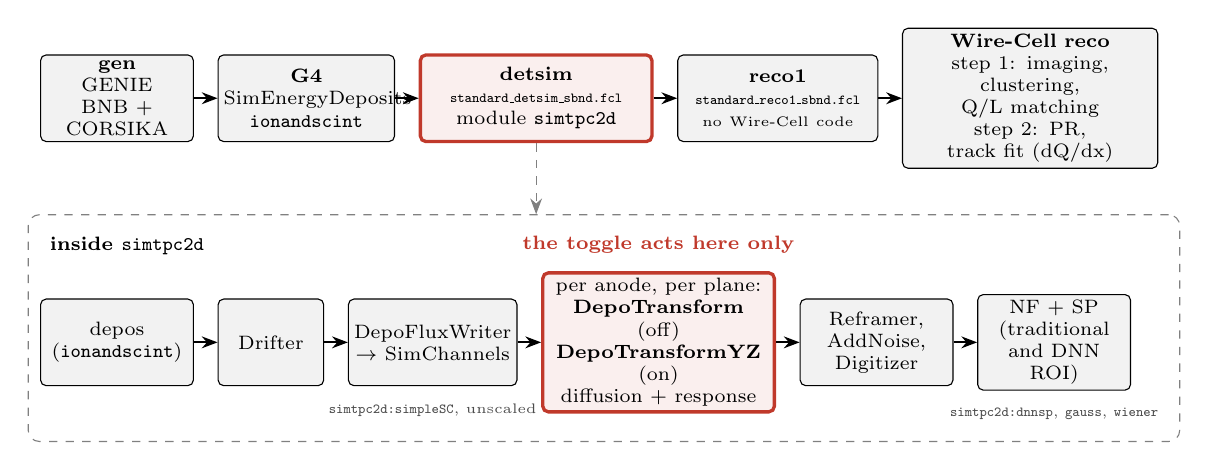
\begin{tikzpicture}[
  stage/.style={draw, rounded corners=2pt, fill=boxbg, align=center, font=\scriptsize,
                minimum height=11mm, text width=20mm, inner sep=2pt},
  act/.style={stage, draw=yz, very thick, fill=yz!8},
  arr/.style={-{Stealth[length=2mm]}, thick},
  note/.style={font=\tiny, align=center, text=black!70}]
\node[stage, text width=18mm] (gen) {\textbf{gen}\\GENIE BNB +\\CORSIKA};
\node[stage, right=3mm of gen, text width=21mm] (g4) {\textbf{G4}\\SimEnergyDeposits\\\code{ionandscint}};
\node[act, right=3mm of g4, text width=28mm] (det) {\textbf{detsim}\\{\tiny\code{standard\_detsim\_sbnd.fcl}}\\module \code{simtpc2d}};
\node[stage, right=3mm of det, text width=24mm] (reco1) {\textbf{reco1}\\{\tiny\code{standard\_reco1\_sbnd.fcl}}\\{\tiny no Wire-Cell code}};
\node[stage, right=3mm of reco1, text width=31mm] (wc) {\textbf{Wire-Cell reco}\\step 1: imaging,\\clustering, Q/L matching\\step 2: PR,\\track fit (dQ/dx)};
\draw[arr] (gen) -- (g4); \draw[arr] (g4) -- (det); \draw[arr] (det) -- (reco1); \draw[arr] (reco1) -- (wc);
% expansion of simtpc2d
\begin{scope}[yshift=-31mm]
\node[stage, text width=18mm] (dep) {depos\\(\code{ionandscint})};
\node[stage, right=3mm of dep, text width=12mm] (dr) {Drifter};
\node[stage, right=3mm of dr, text width=20mm] (flux) {DepoFluxWriter\\$\to$ SimChannels};
\node[act, right=3mm of flux, text width=28mm] (dt) {per anode, per plane:\\\textbf{DepoTransform} (off)\\\textbf{DepoTransformYZ} (on)\\diffusion + response};
\node[stage, right=3mm of dt, text width=18mm] (sn) {Reframer,\\AddNoise,\\Digitizer};
\node[stage, right=3mm of sn, text width=18mm] (sp) {NF + SP\\(traditional\\and DNN ROI)};
\draw[arr] (dep) -- (dr); \draw[arr] (dr) -- (flux); \draw[arr] (flux) -- (dt); \draw[arr] (dt) -- (sn); \draw[arr] (sn) -- (sp);
\node[note, below=1mm of flux] (n1) {\code{simtpc2d:simpleSC}, unscaled};
\node[note, below=1mm of sp] (n2) {\code{simtpc2d:dnnsp}, \code{gauss}, \code{wiener}};
\node[font=\scriptsize\bfseries, text=yz, above=1mm of dt] (tg) {the toggle acts here only};
\node[font=\scriptsize\bfseries, anchor=north west] at ($(dep.north west)+(0,9mm)$) (lab) {inside \code{simtpc2d}};
\end{scope}
\node[draw=gray, dashed, rounded corners, fit=(dep)(sp)(tg)(n1)(n2)(lab), inner sep=1.5mm] (box) {};
\draw[gray, dashed, -{Stealth[length=2mm]}] (det.south) -- (det.south |- box.north);
\end{tikzpicture}}
\vspace{1mm}
\raggedright\small
\begin{itemize}
\item \code{simtpc2d} = Wire-Cell TPC simulation + noise filter (NF) + signal processing (SP) with DNN ROI, in one art module. Optical and CRT simulation in the same detsim job are untouched.
\item Everything after \code{DepoTransform} (noise, NF, SP, products, labels, reco1, Wire-Cell reco) is standard.
\end{itemize}
\end{frame}

% ---------------------------------------------------------------- 4
\begin{frame}[fragile]{The toggle: one fcl parameter}
\lstset{basicstyle=\ttfamily\tiny}
\begin{columns}[T]
\begin{column}{0.48\textwidth}
\footnotesize
\textbf{fcl} (\code{fcl/detsim\_sbnd\_yz.fcl})
\begin{lstlisting}
#include "standard_detsim_sbnd.fcl"
physics.producers.simtpc2d.wcls_main.configs: [
 "pgrapher/experiment/sbnd/wcls-sim-drift-depoflux-nf-sp-yz.jsonnet"]
physics.producers.simtpc2d.wcls_main.params.yz_scaling: "off"
physics.producers.simtpc2d.wcls_main.params.yz_map:
  "sbnd/sbnd-yzmap-run2-gen2-bnblight-v1.json.bz2"
\end{lstlisting}
Wrappers \code{detsim\_sbnd\_yz\_off.fcl} and \code{detsim\_sbnd\_yz\_on.fcl} include it and set \code{yz\_scaling} to \code{"off"} or \code{"on"}.
\vspace{2mm}
\begin{itemize}
\item \textbf{off}: the stock sbndcode v10\_14\_02\_03 Wire-Cell configuration.
\item \textbf{on}: \code{DepoTransform} $\to$ \code{DepoTransformYZ}, plus a \code{YZMap} service.
\item The two jsonnet files are copies of sbndcode's with new names (\code{...-yz.jsonnet}), so they hide nothing of sbndcode. Every change is marked \code{YZ-KIT}.
\item Also changed: three relative imports made absolute (they resolve to the same sbndcode files).
\end{itemize}
\end{column}
\begin{column}{0.5\textwidth}
\footnotesize
\textbf{\code{wcls-sim-drift-depoflux-nf-sp-yz.jsonnet}} vs sbndcode
\begin{lstlisting}[style=diff]
@--local sim_maker = import 'pgrapher/experiment/sbnd/sim.jsonnet';-@
@--local sim = sim_maker(params, tools);-@
@++local yz_scaling = std.extVar('yz_scaling');+@
@++local yzmap = if yz_scaling == 'on' then {+@
@++  type: 'YZMap', name: 'sbnd-yz',+@
@++  data: { filename: std.extVar('yz_map'),+@
@++    nbinsz: 100, nbinsy: 80,+@
@++    bin_width: 5 * wc.cm, bin_height: 5 * wc.cm,+@
@++    zoffset: 0 * wc.cm, yoffset: 200 * wc.cm },+@
@++} else null;+@
@++local sim_maker = import 'pgrapher/experiment/sbnd/sim-yz.jsonnet';+@
@++local sim = sim_maker(params, tools, yzmap);+@
\end{lstlisting}
\vspace{1mm}
\textbf{\code{sim-yz.jsonnet}} vs sbndcode \code{sim.jsonnet}
\begin{lstlisting}[style=diff]
@--function(params, tools) {-@
@++function(params, tools, yzmap=null) {+@
  ...
  local transforms = [
@++  if yzmap == null then+@
      sim.make_depotransform("depotransform-"+tools.anodes[n].name, ...)
@++  else make_depotransform_yz("depotransformyz-"+tools.anodes[n].name,+@
@++                             ..., yzmap)+@
      for n in std.range(0, nanodes-1)],
\end{lstlisting}
\scriptsize Condensed; \code{make\_depotransform\_yz} = the \code{DepoTransform} settings + \code{yzmap}, \code{yzmap\_key}. Full diff: README section 2.
\end{column}
\end{columns}
\end{frame}

% ---------------------------------------------------------------- 5
\begin{frame}[fragile]{``off'' is stock sbndcode: how it is proven}
\small
\code{scripts/check-config-identity.sh <outdir>} (no lar event loop; about 1 minute):
\begin{enumerate}
\item \code{lar -{}-debug-config} on \code{standard\_detsim\_sbnd.fcl} (stock), \code{detsim\_sbnd\_yz\_off.fcl}, \code{detsim\_sbnd\_yz\_on.fcl}.
\item \code{scripts/fcl\_wcls\_args.py} turns \code{simtpc2d.wcls\_main} into \code{wcsonnet} arguments, as larwirecell's WCLS tool does (params $\to$ \code{-V}, structs $\to$ \code{-C}).
\item \code{wcsonnet} compiles each to JSON with the same \code{WIRECELL\_PATH}; key-sorted copies are compared.
\end{enumerate}
\vspace{1mm}
\begin{columns}[T]
\begin{column}{0.47\textwidth}
\textbf{Expected} (README section 7)
\begin{itemize}
\item stock vs off: must print \code{IDENTICAL}.
\item stock vs on: only \code{DepoTransform} $\to$ \code{DepoTransformYZ} (same settings + \code{yzmap}) for the two anodes, a new \code{YZMap}, and the renamed nodes in the graph.
\end{itemize}
\end{column}
\begin{column}{0.5\textwidth}
\textbf{Kit validation run, 2026-11-24} (\code{kit-validation/config-check})
\begin{itemize}
\item stock and off: 660,931 bytes each, same sha256 (\code{b3ba9294dc9d43c5...}).
\item on: 661,293 bytes. The diff is 54 lines: the \code{YZMap} block, \code{yzmap: "YZMap:sbnd-yz"} and \code{yzmap\_key: ""} in \code{depotransformyz-apa0/apa1}, and the graph node names.
\end{itemize}
\end{column}
\end{columns}
\vspace{2mm}
\footnotesize\color{black!70}
Note: off = stock \emph{configuration}, but run on the branch Wire-Cell libraries, which are newer than the CVMFS ones (0.32.1). So ``off'' is not bit-identical to a CVMFS sbndcode detsim. Compare on vs off from the kit.
\end{frame}

% ---------------------------------------------------------------- 6
\begin{frame}[fragile]{The map}
\begin{columns}[T]
\begin{column}{0.5\textwidth}
\footnotesize
\begin{itemize}
\item File (wire-cell-data master, acbe8e5, 80\,kB):\\{\scriptsize\code{sbnd/sbnd-yzmap-run2-gen2-bnblight-v1.json.bz2}}
\item Made from \code{CzyHist\_<plane>\_<tpc>} of\\{\tiny\code{run\_2\_gen\_2\_BNBLight\_data\_v10\_14\_02\_02\_200usEast80usWest.root}}
\item Factor $g = 1/C$, normalized to mean 1 per plane and TPC over the pixels with data (\code{inv-norm}): overall charge scale kept.
\item Empty pixels ($C=0$; East V 52, East Y 80) $\to$ 1. Others as measured, edges included. Range 0.42--1.68.
\item 100 z $\times$ 80 y bins of 5\,cm; z 0--500\,cm, y $-$200 to 200\,cm.
\item Keys: \code{AnodePlane:apa0} = East (TPC 0, $x<0$), \code{apa1} = West; planes \code{"0"}, \code{"1"}, \code{"2"} = U, V, Y.
\end{itemize}
\end{column}
\begin{column}{0.48\textwidth}
\centering
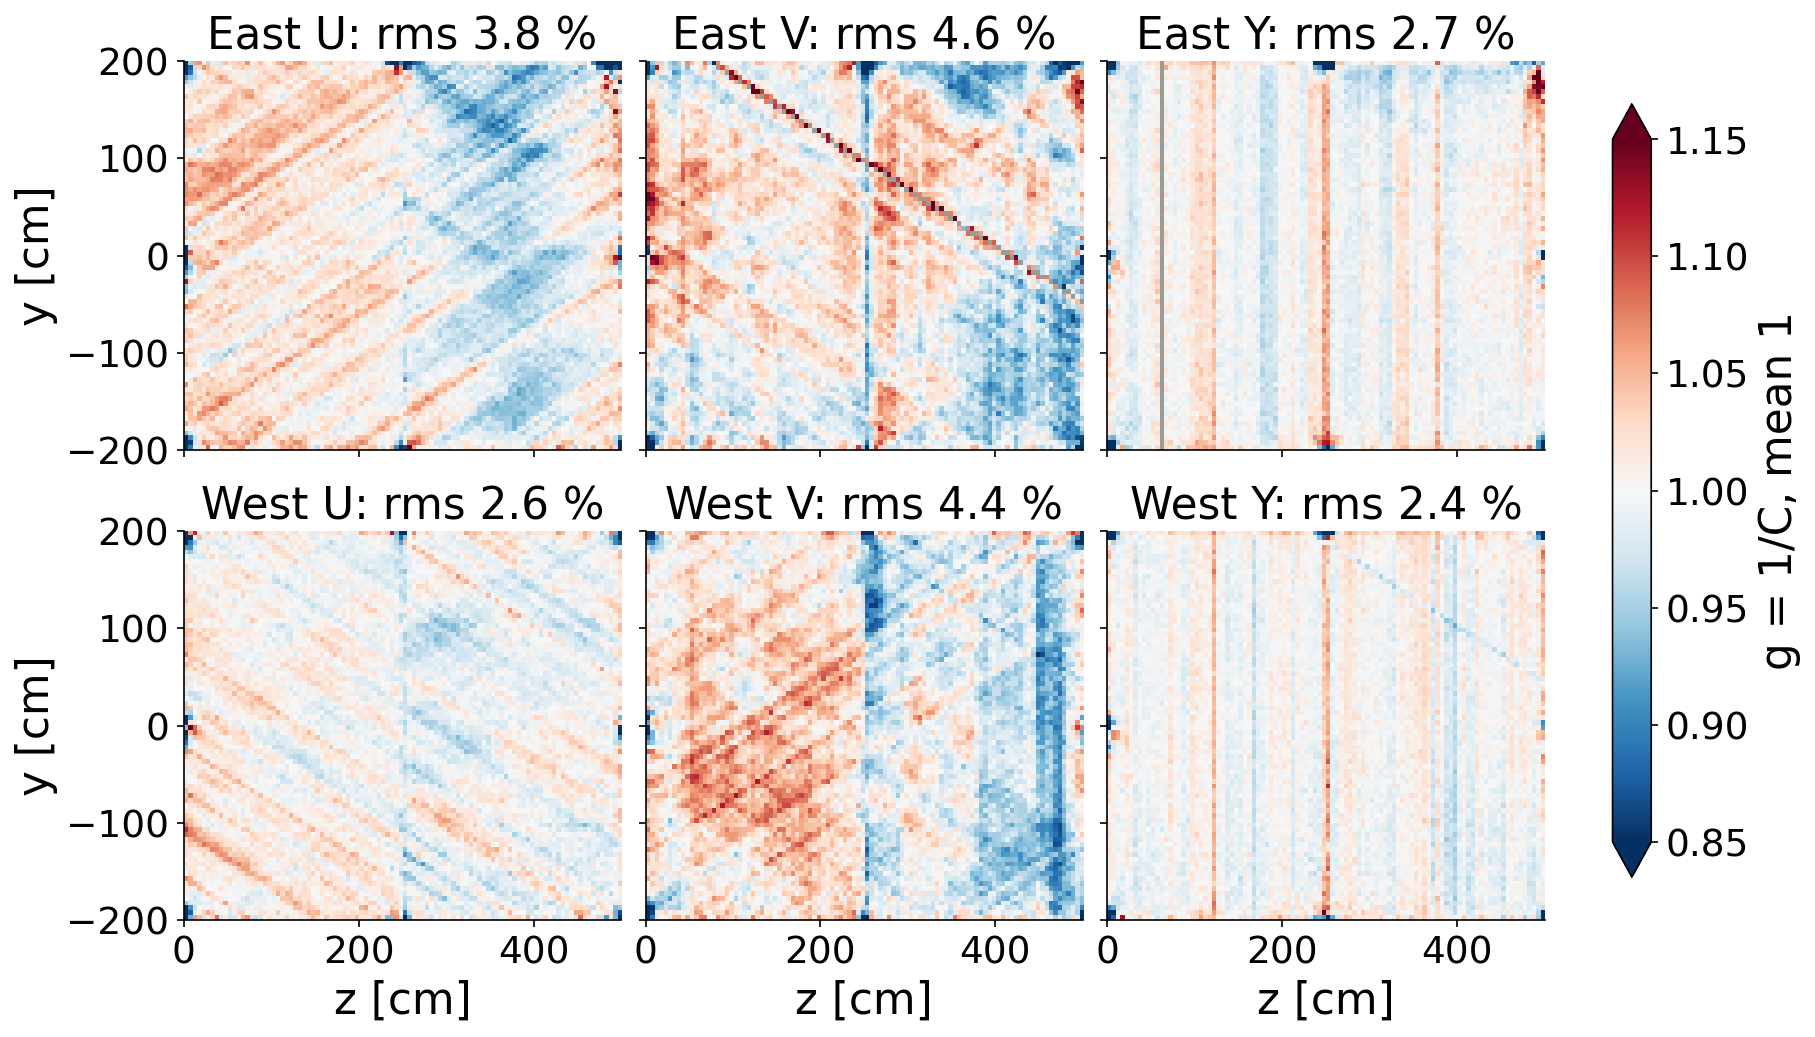
\includegraphics[width=0.92\textwidth]{fig_g_maps.png}\\
\scriptsize From the companion deck: $g$ normalized to mean 1. Gray: no data (factor 1 in the simulation).\\[2mm]
\raggedright\footnotesize
\textbf{Make a new map} (python with numpy + uproot):
\begin{lstlisting}
python3 convert-yzmap-sbnd.py my_calib.root \
    my-yzmap.json.bz2 [--factor inv-norm|inv]
run-yz-detsim.sh --yz on --map my-yzmap.json.bz2 \
    my_g4.root out/on-mymap
\end{lstlisting}
Converter: \code{gen/test/convert-yzmap-sbnd.py} in the branch. It prints the matching binning; another binning needs the \code{YZMap} block changed (copy the kit first).
\end{column}
\end{columns}
\end{frame}

% ---------------------------------------------------------------- 7
\begin{frame}[fragile]{Environment}
\footnotesize
\begin{columns}[T]
\begin{column}{0.5\textwidth}
\textbf{Needed}
\begin{itemize}
\item sbndcode v10\_14\_02\_03 (e26:prof) from CVMFS: fcl, services, cfg, data. SL7 container \code{fnal-dev-sl7}.
\item Wire-Cell libraries of branch \code{sbnd-yz-depo-scaling}: only it has \code{DepoTransformYZ}.
\item larwirecell v10\_01\_28 built against that newer Wire-Cell (branch \code{sbnd-wc-flatcaf}). The CVMFS larwirecell is built against Wire-Cell 0.32.1.
\end{itemize}
\textbf{Why \code{LD\_PRELOAD}}
\begin{itemize}
\item larwirecell has an RPATH to the Wire-Cell it was built with, and RPATH wins over \code{LD\_LIBRARY\_PATH}.
\item So the detsim job runs with \code{LD\_PRELOAD=\$WCT\_YZ\_PRELOAD}: the 14 branch libraries, by bare name. Then every Wire-Cell library comes from the branch, once (checked in \code{/proc/<pid>/maps}).
\item Set it per \code{lar} command; do not export it. \code{run-yz-detsim.sh} does this.
\end{itemize}
\end{column}
\begin{column}{0.48\textwidth}
\textbf{Route A: use our build} (read-only, nothing to build)
\begin{itemize}
\item \code{YZ\_WCT\_LIB}: \code{/exp/sbnd/app/users/yuhw/opt-yz/lib}
\item \code{YZ\_LWC\_DIR}: \code{/exp/sbnd/app/users/yuhw/opt/}\\\code{larwirecell/v10\_01\_28}
\item \code{YZ\_MAP\_PATH}: \code{/exp/sbnd/app/users/yuhw/wire-cell-data}
\item README: ``All of these are readable by every user. You need nothing else.'' If we rebuild it, we will tell you.
\end{itemize}
\textbf{Route B: build it yourself}
\begin{itemize}
\item B1, Wire-Cell only (simplest): \code{scripts/build-wct-yz.sh <src> <prefix> 8}, then \code{export YZ\_WCT\_LIB=<prefix>/lib}. $\sim$9\,GB source + build, $\sim$2\,GB install, 12\,min with 12 jobs.
\item B2, also larwirecell (\code{sbnd-wc-flatcaf}, mrb, larsoft v10\_14\_02): only to change larwirecell; then \code{export YZ\_LWC\_DIR=<product dir>}.
\end{itemize}
\end{column}
\end{columns}
\end{frame}

% ---------------------------------------------------------------- 8
\begin{frame}[fragile]{Run it, step by step}
\footnotesize
The kit (readable by everyone; copy it to change it):
\begin{lstlisting}
K=/exp/sbnd/data/users/yuhw/wire-cell-toolkit-ai-helper/issues/46-sbnd-yz-depo-scaling/yz-sim-kit
\end{lstlisting}
\begin{enumerate}
\item \textbf{Run the same g4 file twice}, one output directory per mode. \code{run-yz-detsim.sh} starts the SL7 container and sources \code{setup-yz-env.sh} by itself:
\begin{lstlisting}
$K/run-yz-detsim.sh --yz off  my_g4.root  out/off  [nevents]
$K/run-yz-detsim.sh --yz on   my_g4.root  out/on   [nevents]
\end{lstlisting}
Options: \code{-{}-reco1} (also runs \code{standard\_reco1\_sbnd.fcl}), \code{-{}-nskip N}, \code{-{}-map FILE} (with \code{-{}-yz on}).
\item \textbf{Check that it worked} (slide 11):
\begin{lstlisting}
apptainer exec -B /cvmfs,/exp,/pnfs,/tmp,/opt \
    /cvmfs/singularity.opensciencegrid.org/fermilab/fnal-dev-sl7:latest bash
source $K/setup-yz-env.sh
python3 $K/scripts/check_yz_scaling.py out/off/detsim/detsim.root out/on/detsim/detsim.root \
    $YZ_MAP_PATH/sbnd/sbnd-yzmap-run2-gen2-bnblight-v1.json.bz2 out/check
$K/scripts/check-config-identity.sh out/config-check
\end{lstlisting}
\item \textbf{By hand} (inside the container, after the setup):
\begin{lstlisting}
LD_PRELOAD=$WCT_YZ_PRELOAD lar -c detsim_sbnd_yz_on.fcl -s g4.root -o detsim.root
\end{lstlisting}
\end{enumerate}
\vspace{1mm}
The two modes can run at the same time, but in different directories: two art jobs in one directory on CephFS (\code{/exp}) fail with ``disk I/O error'' (art's MemoryTracker SQLite file). The script does not overwrite an existing \code{detsim.root}.
\end{frame}

% ---------------------------------------------------------------- 9
\begin{frame}{Inputs: your own G4 or ours}
\small
\textbf{Your own}: any SBND g4 file made with sbndcode v10\_14, with \code{ionandscint} SimEnergyDeposits (as the standard detsim needs).
\vspace{2mm}

\textbf{Ours} (sbndcode v10\_14\_02\_03 e26:prof from CVMFS):
\vspace{1mm}
\centering\footnotesize
\begin{tabular}{@{}>{\raggedright\arraybackslash}p{0.13\textwidth}>{\raggedright\arraybackslash}p{0.38\textwidth}>{\raggedright\arraybackslash}p{0.44\textwidth}@{}}
\toprule
sample & file & how it was made \\
\midrule
BNB CV-like (10+ events) & \code{/exp/sbnd/data/users/yuhw/}\newline\code{YZ-non-uniformity/bnb-cv-10/g4.root}\newline\open{in production; not there yet on 2026-11-25} &
GENIE BNB $\nu$ + CORSIKA cosmics, rockbox: {\scriptsize\code{prodgenie\_corsika\_proton\_rockbox0p1\_sbnd.fcl}}, 70 generated (the rockbox filter keeps $\sim$20\,\%), then \code{standard\_g4\_rockbox\_sbnd.fcl}. The detsim tests use the first 10. \\
\addlinespace
long muons (10 events) & \code{/exp/sbnd/data/users/yuhw/}\newline\code{YZ-non-uniformity/mu-test/g4.root} &
5\,GeV $\mu^-$, start at z = $-$5\,cm, x over $\pm$180\,cm, y over $\pm$120\,cm, along +z ($\pm$20$^\circ$ in YZ, $\pm$3$^\circ$ in XZ), then \code{standard\_g4\_sbnd.fcl}. \\
\bottomrule
\end{tabular}
\raggedright\small
\vspace{2mm}
\begin{itemize}
\item Long muons: cross many YZ pixels on all planes, good for the per-channel check.
\item BNB CV-like: the planned dQ/dx and resource test (placeholders at the end).
\end{itemize}
\end{frame}

% ---------------------------------------------------------------- 10
\begin{frame}[fragile]{Outputs and product labels}
\small
\begin{columns}[T]
\begin{column}{0.41\textwidth}
\textbf{Files} (per mode)
\begin{lstlisting}
out/<mode>/detsim/
  detsim.root   art file, process DetSim
  detsim.log    lar output
  detsim.cmd    the command
  detsim.time   /usr/bin/time -v
  summary.txt   wall, max RSS, art's
                Time/MemoryTracker tables
  timing.db, memory.db   per-module SQLite
out/<mode>/reco1/        with --reco1
  reco1.root + the same files
\end{lstlisting}
\vspace{1mm}
No RawDigits, as in the standard detsim.
\end{column}
\begin{column}{0.57\textwidth}
\textbf{Wire-Cell products in \code{detsim.root}} (all standard)\\[1mm]
\scriptsize
\begin{tabular}{@{}lll@{}}
\toprule
label & type & what \\
\midrule
\code{simtpc2d:dnnsp} & \code{recob::Wire} & SP, DNN ROI \\
\code{simtpc2d:gauss} & \code{recob::Wire} & SP, traditional ROI \\
\code{simtpc2d:wiener} & \code{recob::Wire} & SP, traditional ROI \\
\code{simtpc2d:wiener} & channel summary & SP threshold \\
\code{simtpc2d:bad} & channel mask & bad channels \\
\code{simtpc2d:simpleSC} & \code{sim::SimChannel} & true electrons, \textbf{not scaled} \\
\bottomrule
\end{tabular}
\vspace{2mm}
\small
\begin{itemize}
\item \code{dnnsp} is what production Wire-Cell reco and reco1 \code{gaushit} use.
\item The YZ scaling shows up in \code{dnnsp}, \code{gauss}, \code{wiener} and everything after them; not in \code{simpleSC}.
\end{itemize}
\end{column}
\end{columns}
\end{frame}

% ---------------------------------------------------------------- 11
\begin{frame}{Check that it worked: \code{check\_yz\_scaling.py}}
\small
\begin{columns}[T]
\begin{column}{0.52\textwidth}
Inputs: the off and on detsim files of the \emph{same} g4 events, and the map. About 1 minute for 10 events; PyROOT; no \code{LD\_PRELOAD}.
\vspace{1mm}

Per channel with $\ge$20,000 SimChannel electrons and SP charge in both files:
\begin{itemize}
\item \textbf{predicted} = map value of the channel's plane and TPC at its SimChannel deposits (y, z), weighted by electrons;
\item \textbf{measured} = channel's SP charge (all ROIs), on / off.
\end{itemize}
Per plane and TPC, for \code{dnnsp} and \code{gauss}: channels, rms of predicted, median and rms of measured/predicted $-$ 1, its 5--95\,\% range, correlation, plane totals.
Output: table on stdout, \code{yzcheck.json}, \code{yzcheck.png}, \code{yzcheck\_<product>.tsv}.
\end{column}
\begin{column}{0.45\textwidth}
\textbf{What to expect} (README, long muons)
\begin{itemize}
\item Median of measured/predicted $-$ 1 within about $\pm$0.3\,\% on every plane.
\item Collection: rms $\sim$0.5--1\,\%, correlation $>$0.9.
\item Induction: noisier per channel (a few \% rms), but follows the map on average.
\item ``on = off'' (ratio 1 everywhere, correlation $\sim$0): the scaling did not run.
\end{itemize}
\vspace{2mm}
\textbf{Script cross-check} (kit validation, 2026-11-24): on the earlier toolkit-config long-muon files (next slide) it reproduces the doc-section-3 numbers (18,489 channels; East U median $-$0.01\,\%, corr 0.83; East Y corr 0.93).
\end{column}
\end{columns}
\end{frame}

% ---------------------------------------------------------------- 12
\begin{frame}{Validation so far}
\footnotesize
\textbf{Earlier test, toolkit configuration} (doc section 3, 2026-11-13, rebase check 2026-11-24): 10 long muons, detsim nominal vs yzmap, same opt-yz build, TPC only, traditional ROI (the toolkit jsonnet has no DNN ROI). Measured = SP \code{gauss} charge ratio; 18,489 channel-events used.
\vspace{1mm}
\begin{columns}[T]
\begin{column}{0.53\textwidth}
\centering\setlength{\tabcolsep}{3pt}
\begin{tabular}{@{}lrrrrr@{}}
\toprule
 & chan. & pred. rms & meas/pred $-$1 & rms & corr \\
 & & & median & & \\
\midrule
East U & 4150 & 3.5\,\% & $-$0.01\,\% & 2.2\,\% & 0.83 \\
East V & 6298 & 3.8\,\% & $-$0.13\,\% & 3.0\,\% & 0.74 \\
East Y & 2404 & 1.9\,\% & +0.00\,\% & 0.75\,\% & 0.93 \\
West U & 2228 & 2.3\,\% & $-$0.01\,\% & 2.6\,\% & 0.65 \\
West V & 2274 & 4.4\,\% & $-$0.10\,\% & 3.5\,\% & 0.73 \\
West Y & 1135 & 1.8\,\% & +0.01\,\% & 0.49\,\% & 0.96 \\
\bottomrule
\end{tabular}
\raggedright
\begin{itemize}
\item Each plane follows its own map: median $\le$0.13\,\%; plane totals within 0.3\,\%.
\item Doctest: 5/5 cases, 412 assertions (per-plane ratios equal within $10^{-4}$; unit map = \code{DepoTransform}).
\end{itemize}
\end{column}
\begin{column}{0.45\textwidth}
\centering
\includegraphics[width=\textwidth]{detsim_scaling_rebase.png}\\[1mm]
\raggedright
\textbf{Kit test, sbndcode configuration} (DNN ROI, full detsim):
\begin{itemize}
\item config identity: done (slide 5).
\item 10 long muons, on vs off, \code{check\_yz\_scaling.py}: \open{running; README section 10 not filled yet.}
\end{itemize}
\end{column}
\end{columns}
\end{frame}

% ---------------------------------------------------------------- 13
\begin{frame}{Placeholder: deconvolved dQ/dx, 10-event BNB CV-like test}
\placeholder{Truth-track SP dQ/dx per plane (U, V, Y) and TPC, on vs off; ratio vs the map.}
\small
\textbf{Planned method}
\begin{itemize}
\item Input: \code{bnb-cv-10/g4.root}, first 10 events, detsim on and off (same g4, same libraries).
\item Truth-track SP dQ/dx, per wire and per plane: SP charge (\code{simtpc2d:dnnsp}) in a window around the true track on that wire, divided by the track's 3D length seen by that wire. As in the dQ/dx data/MC note of \code{Ningclover/sbnd-wirecell-bdt} (\code{docs/dqdx\_data\_mc.md}).
\item Because both modes start from the same depos and SimChannels, on/off per wire isolates the YZ scaling.
\item To show: on/off ratio vs y and z per plane, and vs the map's $g$ at the track position; the 1D dQ/dx per plane, on and off.
\end{itemize}
\end{frame}

% ---------------------------------------------------------------- 14
\begin{frame}{Placeholder: fitted dQ/dx after the full Wire-Cell reconstruction}
\placeholder{Fitted dQ/dx from Wire-Cell TrackFitting, on vs off, same 10 events.}
\small
\textbf{Planned method}
\begin{itemize}
\item Run the standard Wire-Cell reco on both detsim outputs: step 1 (imaging, clustering, Q/L matching), step 2 (pattern recognition and track fitting).
\item Take the fitted dQ/dx per track point from Wire-Cell \code{TrackFitting}; compare on vs off for matched tracks, vs y and z.
\item Question this answers: how much of the per-plane YZ structure survives in the fitted dQ/dx that analyses use.
\end{itemize}
\end{frame}

% ---------------------------------------------------------------- 15
\begin{frame}{Placeholder: computing resources}
\placeholder{detsim wall time, \code{simtpc2d} module time per event (art TimeTracker), max RSS; on vs off; 10 BNB CV-like events.}
\small
\textbf{How}: \code{run-yz-detsim.sh} writes \code{detsim.time} (\code{/usr/bin/time -v}), \code{summary.txt}, \code{timing.db} and \code{memory.db} for each mode.
\vspace{1mm}

\textbf{Known so far} (not the BNB test)
\begin{itemize}
\item Toolkit configuration, 10 long muons, TPC only: nominal 4:55, yzmap 4:56 wall; 1.9\,GB peak RSS (doc section 3). The scaling costs no measurable time.
\item Kit (full sbndcode detsim with DNN ROI), 1 long muon incl. start-up: 2:23 wall, 6.1\,GB max RSS (kit smoke test, 2026-11-24).
\item README: \code{simtpc2d} (Wire-Cell sim + NF + SP + DNN ROI on CPU) is most of the time; one job is single-threaded at the art level; give it $\sim$7\,GB of memory.
\end{itemize}
\end{frame}

% ---------------------------------------------------------------- 16
\begin{frame}{Caveats, open questions, contacts}
\footnotesize
\begin{columns}[T]
\begin{column}{0.52\textwidth}
\textbf{Caveats}
\begin{itemize}
\item ``off'' = stock sbndcode configuration on newer Wire-Cell libraries. Compare on vs off from the kit, not on vs a CVMFS sbndcode detsim.
\item SimChannels are not scaled. Anything that uses SimChannel charge as ``expected reco charge'' sees the map as a reco/true difference.
\item The map is from data (Run 2, gen2, BNB Light) and keeps all it measured, incl. dead-channel stripes and edge pixels with large corrections (11--15 pixels per plane with $C>1.3$, all in the outer 10\,cm, 870--1,210 hits median). Dead channels in the sim come from the channel status, not the map.
\item The kit depends on our read-only install (route A); route B makes you independent.
\end{itemize}
\end{column}
\begin{column}{0.45\textwidth}
\textbf{Open questions for the map author}
\begin{itemize}
\item Unit and calibration stage of \code{zy} (ADC/cm?).
\item What ``200usEast80usWest'' means.
\item The \code{\_0}/\code{\_1} index of \code{dqdxHist} (both hold East + West hits).
\item An MC version of the same histograms (data vs MC is open).
\item The outer-10\,cm pixels: keep, cap or fill? (the converter is the place).
\item Event selection and run range; \code{zydqdx}.
\end{itemize}
\vspace{2mm}
\textbf{Contacts}
\begin{itemize}
\item Wire-Cell simulation, the kit, the converter: Haiwang Yu (BNL).
\item The YZ map: its author, SBND calibration.
\item Issue log: \code{46-sbnd-yz-depo-scaling.md}.
\end{itemize}
\end{column}
\end{columns}
\end{frame}

\end{document}
